\chapter{Taylors sætning anvendt på trigonometriske funktioner og enhedscirklen}
Dette kapitel vil vise, hvordan man anvender den før redegjort for teori på trigonometriske funktioner og til at tilnærme sig $\pi$. Målet er at vise, hvordan man numerisk kan udregne værdier for $\sin(x)$, $\cos(x)$ og $\tan(x)$, samt hvordan man kan anvende enhedscirklen og Taylorpolynomier til at finde en approksimation $\pi$.
\section{Taylorrække for $\sin(x)$}
Når man udleder en Taylorrække, så er det værd at tænke på, hvilken $a$-værdi man vælger, da den ofte afgør, hvor nyttig Taylorrækken er. Målet med Taylorrækken er at gøre $\sin(x)$ nemmere at regne på, så ideelt vil man blandt $\sin(x)$ og dens afledte finde værdier for $a$, der giver heltal eller nemme brøker. Først differentieres $\sin(x)$, så man kan skabe sig et overblik over de afledte til funktionen;
\begin{align*}
f(x) &= \sin(x) \\
f'(x) &= \cos(x) \\
f''(x) &= -\sin(x) \\
f^{(3)}(x) &= -\cos(x) \\
\end{align*}
Sinusfunktionens afledte bliver ved med at svinge mellem positiv og negativ $\sin(x)$ og $\cos(x)$. Hvis man ser på enhedscirklen, så vil funktionerne alle give heltal for hver kvarte omgang fra startpunktet $(0,0)$, hvilket svarer værdier af $1/2\pi$ ganget med et heltal $z$, hvor $z\in\mathbb{Z}$. Hvis $a=1/2\pi z$, så giver $\sin(x)$ og dens afledte pæne værdier i form af heltallene $-1$, $0$ og $1$. Dog så vil Taylorrækken indeholde $\pi$ for alle $z \neq 0$, hvilket kan gøre udregninger senere svære. Derfor vælges $z=0$ og dermed $a=0$, hvilket giver følgende værdier for $\sin(x)$ og dens afledte;
\begin{align*}
\sin(0) &= 0 \\
\cos(0) &= 1 \\
-\sin(0) &= 0 \\
-\cos(0) &= -1 \\
\end{align*}
Taylorrækken for $\sin(x)$ omkring $0$ bliver derfor;
\begin{align*}
T_{\sin} (x) &= 0+x+0 \cdot \frac{x^2}{2}-\frac{x^3}{3!}+0 \cdot \frac{x^4}{4!}+\frac{x^5}{5!}+... 
\\
T_{\sin} (x) &= x-\frac{x^3}{3!}+\frac{x^5}{5!}+... \\
\end{align*}
%kilde til ulige funktioners maclaurinrækker
Siden $\sin(x)$ er en ulige funktion, da $\sin(x)=-\sin(-x)$, så er $f^{n}(0)=0$, hvis $n \mod 2=0$. Dermed er det kun de led, hvor $x$ er opløftet i en ulige eksponent, tilbage, hvor eksponenten kan udtrykkes som $2n+1$, for $n\in \mathbb{N}_0$. De resterende led skrifter mellem at være positive $1$ og negative $1$. Her ses det, at leddet $n=0$ er positivt, dermed kan man indfører $(-1)^n$ for at sikre, at leddene skifter mellem at være positive og negative i rigtig rækkefølge. Dermed bliver summen for Taylorrækken for $\sin(x)$ omkring $0$;
\begin{align*}
T_{\sin}(x)=\sum_{n=0}^{\infty} \frac{(-1)^n}{(2n+1)!}x^{2n+1}
\end{align*}
Der er dog ingen garanti for, at rækken konvergerer med $\sin(x)$. Derfor testes kvotientkriteriet for rækken;
\begin{align*}
\lim\limits_{n \to \infty}
\left\lvert
\frac{\frac{(-1)^{n+1}}{(2(n+1)+1)!}}
{\frac{(-1)^n}{(2n+1)!}} 
\right\lvert
&=
\lim\limits_{n \to \infty}
\left\lvert
\frac{\frac{(-1)^{n+1}}{(2n+3)!}}
{\frac{(-1)^n}{(2n+1)!}}
\right\lvert 
\\
&=
\lim\limits_{n \to \infty}
\frac{\frac{\left\lvert (-1)^{n+1} \right\lvert }{(2n+3)!}}
{\frac{\left\lvert (-1)^n \right\lvert }{(2n+1)!}}
\\
&=
\lim\limits_{n \to \infty}
\frac{\frac{1}{(2n+3)!}}
{\frac{1}{(2n+1)!} }
\\
&=
\lim\limits_{n \to \infty}
\frac{1}{(2n+3)!}
\cdot
\frac{(2n+1)!}{1}
\\
&=
\lim\limits_{n \to \infty}
\frac{1}{(2n+3)(2n+2)}
=0 \\
\end{align*}
Det viser sig, at rækken konvergerer med $\sin(x)$ for alle $x$'er, da $r=\infty$, hvor $r$ er konvergensradiussen.
\begin{equation}\label{eq:sinrække}
\sin(x)=\sum_{n=0}^{\infty} \frac{(-1)^n}{(2n+1)!}x^{2n+1}
\end{equation}
Dette er også Maclaurinrækken for $\sin(x)$, da $c=0$. Med rækken kan man danne Maclaurinpolynomier, hvor der herunder er plottet nogle Maclaurinpolynomiet for at visualisere, hvordan de approksimerer $\sin(x)$;
\begin{figure}[H]
	\centering
	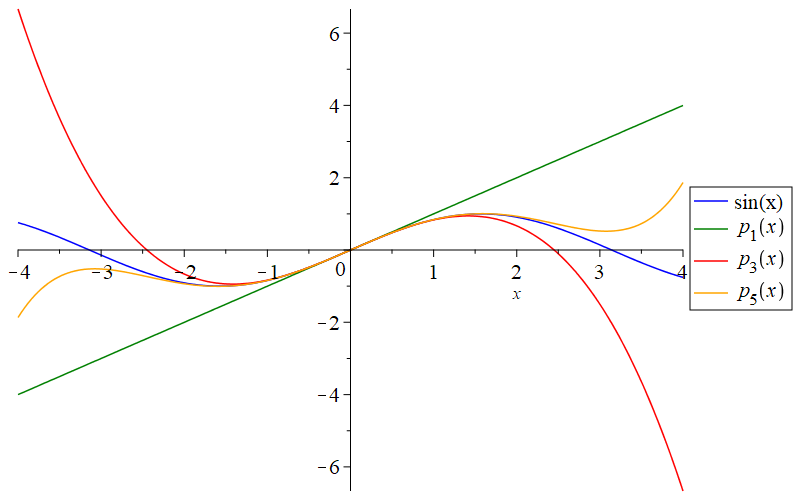
\includegraphics[scale=0.4]{fig/img/taylor_sin}
	\caption{Approksimation af sinus omkring 0 af Maclaurinpolynomier af første, tredje og femte orden}
 	\label{fig:taylor_sin}
\end{figure}
Maclaurinpolynomiet af femte orden kan med god tilnærmelse give værdier for $\sin(x)$ i intervallet $[-\pi /2; \pi /2]$, hvor den absolutte værdi af restleddet maksimalt giver $\left\lvert R_5(\pi/2) \right\lvert = \pi^6/{(6! \cdot 2^6)} = \pi^6/{46080}$. Intervallet dækker en halv svingning, og siden $sin(x)$ svinger harmonisk, så kan man approksimere værdier for $\sin(x)$, der er udenfor intervallet ved at anvende en korresponderende værdi indenfor intervallet. Eksempelvis, så kan man approksimere værdien af $\sin(t)$, hvor $t \in ]\pi/2;\pi]$, ved at udregne $p_5(\pi-t)$, da $\sin(t) = \sin(\pi-t)$. Der er dermed ikke grund til at fremstille et Maclaurinpolynomium af højere orden, da det vil gøre beregningerne sværere.
%referer til eksempel af Esben
\section{Taylorrække for $\cos(x)$}
Hvis man derefter vil udlede en Taylorrække for $\cos(x)$ omkring samme $a$-værdi, så vil man kunne differentiere Taylorrækken for $\sin(x)$, da $\frac{d}{dx}\sin(x)=\cos(x)$. Hvis man differentiere Taylorrækken i ligning \ref{eq:sinrække}, så får man rækken;
%man kan differentiere serien p.ga. teori 19 i calculus-bogen side 536-537 section 9.5
\[
\frac{d}{dx} \sum_{n=0}^{\infty} \frac{(-1)^n}{(2n+1)!}x^{2n+1}
=
\sum_{n=0}^{\infty} \frac{(-1)^n}{(2n)!}x^{2n}
\]
Igen kan man anvende kvotientkriteriet på rækken for at se, om den konvergerer med $\cos(x)$.
\begin{align*}
\lim\limits_{n \to \infty}
\left\lvert
\frac{\frac{(-1)^{n+1}}{(2(n+1))!}}
{\frac{(-1)^n}{(2n)!}} 
\right\lvert
&=
\lim\limits_{n \to \infty}
\left\lvert
\frac{\frac{(-1)^{n+1}}{(2n+2)!}}
{\frac{(-1)^n}{(2n)!}}
\right\lvert 
\\
&=
\lim\limits_{n \to \infty}
\frac{\frac{\left\lvert (-1)^{n+1} \right\lvert }{(2n+2)!}}
{\frac{\left\lvert (-1)^n \right\lvert }{(2n)!}}
\\
&=
\lim\limits_{n \to \infty}
\frac{\frac{1}{(2n+2)!}}
{\frac{1}{(2n)!} }
\\
&=
\lim\limits_{n \to \infty}
\frac{1}{(2n+2)(2n+1)}
=0 \\
\end{align*}
Dermed konvergerer denne række med $\cos(x)$ for alle $x$'er. Rækken er også kendt som Maclaurinrækken for $\cos(x)$;
%evt. kilde til Maclaurinserien for cosinus i bogen side 544-545 section 9.6
\begin{equation}\label{eq:cosrække}
\cos(x)=\sum_{n=0}^{\infty} \frac{(-1)^n}{(2n)!}x^{2n}
\end{equation}
Hvorimod man kunne udlede rækken ved at arbejde med $\cos(x)$, så gjorde de kendte relationer mellem $\cos(x)$ og $\sin(x)$ det nemmere at udlede rækken med den allerede udledte række for $\sin(x)$ i ligning \ref{eq:sinrække}. Maclaurinrækken  for $\sin(x)$ kunne man også integrerer og multiplicerer med $-1$ for at få Maclaurinrækken for $\cos(x)$, da $\int \sin(x) dx=-\cos(x)+k$, hvor $k=-\cos(0)=-1$;
\begin{align*}
-\int \sum_{n=0}^{\infty} \frac{(-1)^n}{(2n+1)!}x^{2n+1} dx
&=
-\left(\sum_{n=1}^{\infty} \frac{(-1)^n}{(2n)!}x^{2n}-1\right) \\
&=
\sum_{n=0}^{\infty} \frac{(-1)^n}{(2n)!}x^{2n} \\
\end{align*}
Den samme række opstår, dermed kan man anvende Maclaurinrækken for $\sin(x)$ til at udlede Maclaurinrækken for $\cos(x)$ ved både differentiation og integration. Igen kan man med Maclaurinrækken danne Maclaurinpolynomier;
\begin{figure}[H]
	\centering
	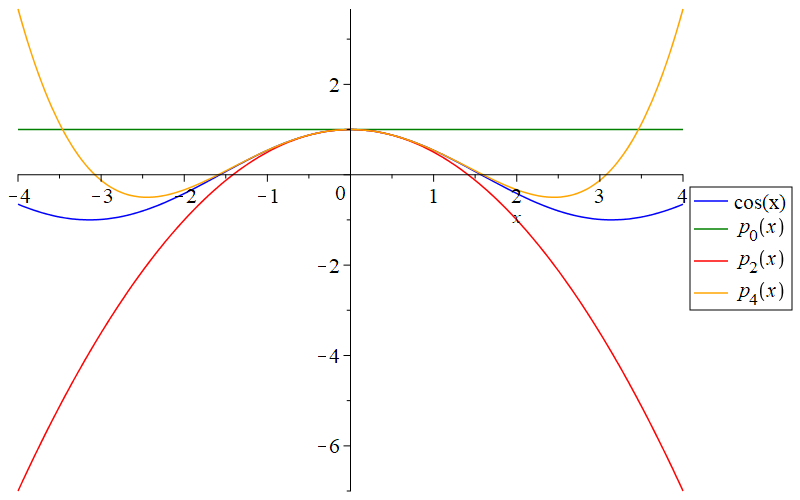
\includegraphics[scale=0.4]{fig/img/taylor_cos}
	\caption{Approksimation af cosinus omkring 0 af Maclaurinpolynomier af nulte, anden og fjerde orden}
 	\label{fig:taylor_cos}
\end{figure}
Mangen til \ref{fig:taylor_sin}, så ses det, at Maclaurinpolynomiet af fjerde orden giver en god tilnærmelse af $\cos(x)$ i intervallet $[-\pi /2; \pi /2]$, hvor den maksimale absolutte værdi af restleddet er $\left\lvert R_4(\pi/2) \right\lvert = \pi^5/(5! \cdot 2^5) = \pi^5/3840$. $[-\pi /2; \pi /2]$ dækker et udsving af $\cos(x)$, hvilket man kan anvende til at finde værdier for $\cos(x)$ udover intervallet, igen mangen til Maclaurinpolynomiet af femte orden for $\sin(x)$.
\section{Approksimation af $\tan(x)$}
Til $\tan(x)$ kan man igen udnytte dens relation til de andre trigonometriske funktioner, hvor ligningen $\tan(x)=\frac{\sin(x)}{\cos(x)}$ er gældende. Hvis man derfor tager rækken i ligning \ref{eq:sinrække} og dividerer med rækken i ligning \ref{eq:cosrække}, så får man $\tan(x)$;
\begin{equation}\label{eq:tanbrøk}
\tan(x)
=
\frac{\sum_{n=0}^{\infty} \frac{(-1)^n}{(2n+1)!}x^{2n+1}}
{\sum_{n=0}^{\infty} \frac{(-1)^n}{(2n)!}x^{2n}}
\end{equation}
Hvis man tager delsumme af de to summe med samme øvre grænse, så for man en rationel funktion, som approksimerer $\tan(x)$ omkring $0$;
\begin{figure}[H]
	\centering
	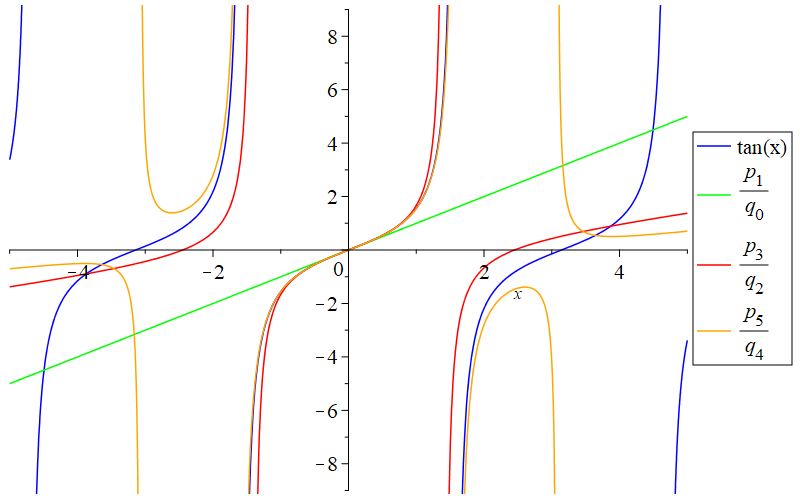
\includegraphics[scale=0.4]{fig/img/approks_tan}
	\caption{Approksimation af tangens omkring 0 via Maclaurinpolynomier af $\sin(x)$, noteret $p_n$, og $\cos(x)$, noteret $q_n$.}
 	\label{fig:approks_tan}
\end{figure}
Approksimationen af tangens går igen tilbage til Maclaurinpolynomierne på \ref{fig:taylor_sin}, da de rationelle funktioner på \ref{fig:approks_tan} kan omformuleres til $R(x)=p_n(x)/p_n'(x)$. Omformuleringen giver også god mening i forhold til gennemgangen, hvor Maclaurinrækken for $\cos(x)$ blev udledt ved at differentiere Maclaurinrækken for $\sin(x)$, så $\tan(x)=\sin(x)/\frac{d}{dx}\sin(x)$. Derfor kan man med et Maclaurinpolynomium for $\sin(x)$ approksimere $\tan(x)$ omkring $0$.
\section{Approksimation af $\pi$}
Taylorpolynomier kan også anvendes, når man skal bestemme en værdi numerisk. En sådan værdi kunne være $\pi$, hvor man anvender, hvordan $\pi$ hænger sammen med andre størrelser i cirkler. En sammenhæng er arealet af en cirkel og radiussen; $A=\pi \cdot r^2$. Her kan man med fordel vælge $r=1$, så $A=\pi$ og cirklen har ligningen $x^2+y^2=1$. Ligningen kan ændres, så man får en funktion over en halvcirkel; $y=g(x)=\sqrt{1-x^2}$. Arealet under funktionen er $\pi/2$, men det er svær at integrere $g(x)$, derfor dannes et Taylorpolynomium over funktionen, og det integreres i stedet for $g(x)$. Til denne funktion og dens afledte findes de pæneste værdier, når $x=0$.
\begin{align*}
g(0) &= 1 \\
g'(0) &= 0 \\
g''(0) &= -1 \\
g^{(3)}(0) &= 0 \\
g^{(4)}(0) &= -3 \\
\end{align*}
Dermed kan man lave et fjerdeordens Maclaurinpolynomium.
\begin{align*}
p_{4} (x) &= 1 + 0\cdot \frac{x}{1!} - 1\cdot \frac{x^2}{2!} + 0\cdot \frac{x^3}{3!} - 3\cdot \frac{x^4}{4!}
\\
p_{4} (x) &= 1-\frac{x^2}{2}-\frac{x^4}{8} \\
\end{align*}
Maclaurinpolynomiet integreres fra $x=-1$ til $x=1$, da funktion, og dermed halvcirklen, er defineret i intervallet [-1;1].
\[
\int_{-1}^{1} 1-\frac{x^2}{2}-\frac{x^4}{8} dx = \frac{97}{60} \approx 1,6167
\]
Resultatet var en tilnærmelse af $\pi/2$, så $2\cdot 1,6167 = 3,2334$ er en tilnærmelse af $\pi$. Tilnærmelsen er dog kun med $1$ korrekt ciffer og ingen korrekte decimaler. 
Hvis der ønskes en bedre approksimation bør antallet af led i Taylorpolynomiet stige, dette er 
imidlertidligt ikke særligt simpelt at lave i hånden, da de afledte hurtigt vokser i kompleksitet, 
se appendix (\ref{app:afledte}).  % REFERE TIL APPENDIX
Derfor blev der udarbejdet et simpelt python program til beregningerne, 
som kunne beregne de afledte op til $n$'te orden og derefter integrere Taylorpolynomiet:
Kildekoden kan ses i appendix (\ref{app:kildeKode}). 
Koden indeholder 2 hoved funktioner:
\begin{itemize}
  \item "computeDerivatives" som beregner de afledte for funktionen $f(x)$ 
  i punktet $a$, dette sker ved hjælp af python pakken SymPy, herefter returneres disse som en liste af værdier.  
  \item "intergrateTaylor" som beregner værdien af intergralet imellem to endepunkter
  og returnerer værdierne for intergralet $\int_{-1}^1 P_N (x) dx$ ved specifike ordener $N$. 
\end{itemize}
Når koden køres fås følgende værdier:
\begin{table}[H]
  \begin{center}
    \begin{tabular}{ |c|c|c|c|c|c|c| }
      \hline
        Antal led $N$ & 10 & 20 & 50 & 100 & 200 & 500 \\
      \hline
        Approksimation & $1,5852$ & $1,5763$ & $1,5723$ & $1,5713$ & $1,5709$ & $1,5708$ \\
      \hline
    \end{tabular}
    \caption{Approksimationen i forhold til ordenen af taylor polynomiet}
  \end{center}
\end{table}
%\label{tab:approksimationenVsN}
Den bedste tilnærmelse af $\pi$ er da $2\cdot 1,5708=3,1416$. Som det kan ses i tabellen sker der en mindre og mindre ændring i værdien for approksimationen når $N$ bliver større og større.
I denne sammenhæng er det også interessant at kigge på fejlen imellem approksimationen $\int_{-1}^1 P_N(x) dx$ og $\frac{\pi}{2}$:
\begin{figure}[H]
  \centering
  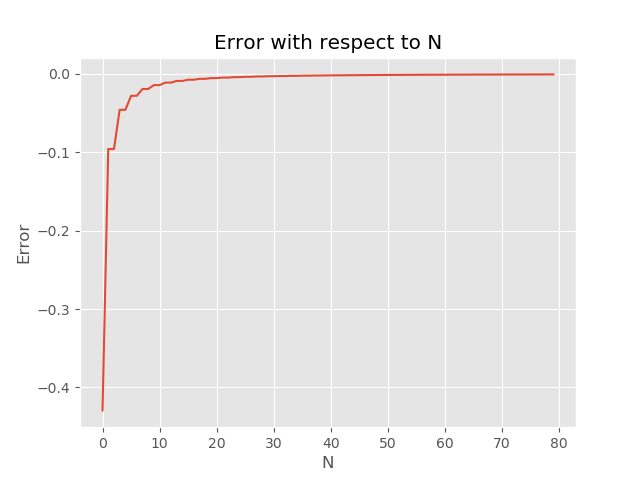
\includegraphics[width=\textwidth]{fig/img/ErrorWithRespectToN.png}
  \caption{Fejl i forhold til antalet af led $N$}
  \label{fig:FejlIForholdTilN}
\end{figure}
Som det kan ses falder fejlen hurtigt i starten når $N$ er lille, men som $N$ vokser flader fejlen ud fordi $P_{N-1}(x) \approx P_{N}(x)$ når $N \rightarrow \infty$.
